% Simulation: Heston model, VIX futures, VIX calls and the convexity adjustment (Daniel).
% Numbers and both tables come from heston/heston_vix.py; checks are in heston/test_heston_vix.py.

\subsubsection{Model and parameters}

Under the risk-neutral measure $\mathbb{Q}$ the Heston model lets the variance $v_t$ of the S\&P~500 move randomly while being pulled back toward a long run level:
\begin{equation}
  dS_t = rS_t\,dt + \sqrt{v_t}\,S_t\,dW^1_t, \qquad
  dv_t = \kappa(\theta - v_t)\,dt + \sigma\sqrt{v_t}\,dW^2_t, \qquad
  \operatorname{corr}(dW^1_t, dW^2_t) = \rho .
  \label{eq:heston}
\end{equation}
Here $S_t$ is the index level and $r$ is the risk-free rate. $W^1$ and $W^2$ are Brownian motions that drive the index and its variance, and their increments have correlation $\rho$. The parameter $\kappa$ is the speed at which $v_t$ returns to the long run variance $\theta$, and $\sigma$ is the volatility of variance. A negative $\rho$ makes volatility rise when the index falls.

The values of $\kappa$, $\theta$, $\sigma$ and $\rho$ come from Gatheral's textbook \cite{gatheral}, where Heston is fitted to S\&P~500 option prices. These describe how variance behaves in general. The starting variance $v_0$ describes one particular day, so we set it from the market's VIX on that day (Section~\ref{sec:hestonvix}). Table~\ref{tab:hestonparams} lists all five. Our prices depend only on $\kappa$, $\theta$, $\sigma$ and $v_0$. The correlation $\rho$ affects the index but not the VIX, which depends on $v_t$ alone (Section~\ref{sec:hestonvix}).

The Feller condition $2\kappa\theta \ge \sigma^2$ guarantees that $v_t$ stays strictly positive. Here $2\kappa\theta = 0.094 < \sigma^2 = 0.150$, so the condition fails and $v_t$ can reach zero. This is why the simulation uses full truncation (Section~\ref{sec:hestonsim}).

\begin{table}[H]
\centering
\small
\begin{tabular}{@{}llrl@{}}
\toprule
\textbf{Parameter} & \textbf{Meaning} & \textbf{Value} & \textbf{Source}\\
\midrule
$\kappa$ & speed of mean reversion (per year) & 1.3253 & Gatheral\\
$\theta$ & long run variance (VIX 18.8) & 0.0354 & Gatheral\\
$\sigma$ & volatility of variance & 0.3877 & Gatheral\\
$\rho$ & correlation of the two shocks & $-0.7165$ & Gatheral (does not affect VIX)\\
$v_0$ & variance on 3 November 2026 & 0.0438 & matched to VIX of 20.83\\
\bottomrule
\end{tabular}
\caption{Heston parameters. Gatheral's values are his fit to the S\&P~500 option surface of 15 September 2005 \cite[Table~3.2]{gatheral}\verify.}
\label{tab:hestonparams}
\end{table}

\subsubsection{The VIX under Heston}
\label{sec:hestonvix}

We first need the variance expected at a future date $s$, seen from today $t$. In the variance equation of \eqref{eq:heston} the random shocks average to zero, so on average each instant closes the same fraction $\kappa$ of the gap between $v$ and $\theta$. The gap is therefore discounted at rate $\kappa$, like a continuously compounded rate, which gives
\begin{equation}
  \EQ_t[v_s] = \theta + (v_t-\theta)\,e^{-\kappa(s-t)}, \qquad s \ge t.
  \label{eq:hestonmean}
\end{equation}
With $\kappa = 1.3253$ the gap halves about every six months.

$\VIX_t^2$ is the risk-neutral expected average variance over the next $\tau = 30/365$ years, so we average \eqref{eq:hestonmean} over that window. The long run part stays $\theta$. The gap part becomes today's gap times $B$, the average of the discount factor $e^{-\kappa u}$ over the 30 days, which is the average share of today's gap still present during the month. This gives an exact formula in $v_t$ alone:
\begin{equation}
  \VIX_t^2 = 100^2\,\EQ_t\!\left[\frac{1}{\tau}\int_t^{t+\tau} v_s\,ds\right]
  = 100^2\left[\theta + (v_t - \theta)\,B\right], \qquad B = \frac{1-e^{-\kappa\tau}}{\kappa\tau} = 0.9475 .
  \label{eq:hestonvix}
\end{equation}
VIX futures and options therefore depend only on $v$. We never simulate $S_t$, and $\rho$ plays no role.

We compare the model with the futures curve of 3 November 2026, the latest date in our futures data. The VIX closed at 20.83 that day. We can observe the VIX but not today's variance $v_0$, so we choose the $v_0$ that makes the model's VIX equal 20.83. Putting $\VIX = 20.83$ into \eqref{eq:hestonvix} and solving gives
\[
  v_0 = \theta + \frac{(20.83/100)^2 - \theta}{B} = 0.0438 .
\]

\subsubsection{Simulation}
\label{sec:hestonsim}

We simulate $v$ forward with an Euler scheme \cite{gatheral}, which replaces the continuous equation by daily steps of pull and random shock. We use $\Delta = 1/365$, 100{,}000 paths and random seed 42, out to 180 days. Because the Feller condition fails, a step can push $v$ below zero, so we use full truncation and replace $v$ by $v^+ = \max(v,0)$ in the pull and under the square root. One step is
\[
  v_{t+\Delta} = v_t + \kappa(\theta - v_t^+)\Delta + \sigma\sqrt{v_t^+\Delta}\;Z, \qquad Z\sim N(0,1),
\]
with a new $Z$ for every path and day. On each date $T$, every path's $v_T$ is converted into a $\VIX_T$ with \eqref{eq:hestonvix}. These simulated values of $\VIX_T$ are used to price the futures and calls below. The Monte Carlo standard error, the typical change in a price if we reran with new random numbers, is at most 0.03 VIX points for futures and 0.02 points for calls.

To test the simulation we compared it with results known in advance. On day 0 the model's VIX is exactly 20.83, the market close on 3 November. The average variance also has an exact formula \eqref{eq:hestonmean}. Table~\ref{tab:hestonchecks} compares it with the simulated average on days 30 and 91, the call maturities, and on day 180, the last simulated day. Every difference is smaller than the random error. Finally, rerunning with 200{,}000 paths changes no price by more than 0.012 points for futures and 0.010 points for calls\unskip.

\begin{table}[H]
\centering
\small
\begin{tabular}{@{}lrrrr@{}}
\toprule
\textbf{Day} & \textbf{Simulated $\EQ[v_T]$} & \textbf{Exact $\EQ[v_T]$} & \textbf{Difference} & \textbf{Random error (2 s.e.)}\\
\midrule
30 & 0.04306 & 0.04296 & +0.24\% & 0.33\% \\
91 & 0.04150 & 0.04146 & +0.10\% & 0.52\% \\
180 & 0.03966 & 0.03979 & -0.31\% & 0.66\% \\
\bottomrule
\end{tabular}

\caption{Simulated against exact average variance. The random error is two standard errors, the range within which about 95\% of reruns would fall.}
\label{tab:hestonchecks}
\end{table}

\subsubsection{Futures curve vs market}

A VIX future pays $\VIX_T$ and costs nothing to enter, so its price is $F(T) = \EQ[\VIX_T]$, the average of $\VIX_T$ over the paths. Figure~\ref{fig:hestoncurve} and Table~\ref{tab:hestonfutures} compare it with the settlements of 3 November 2026.

\begin{figure}[H]
\centering
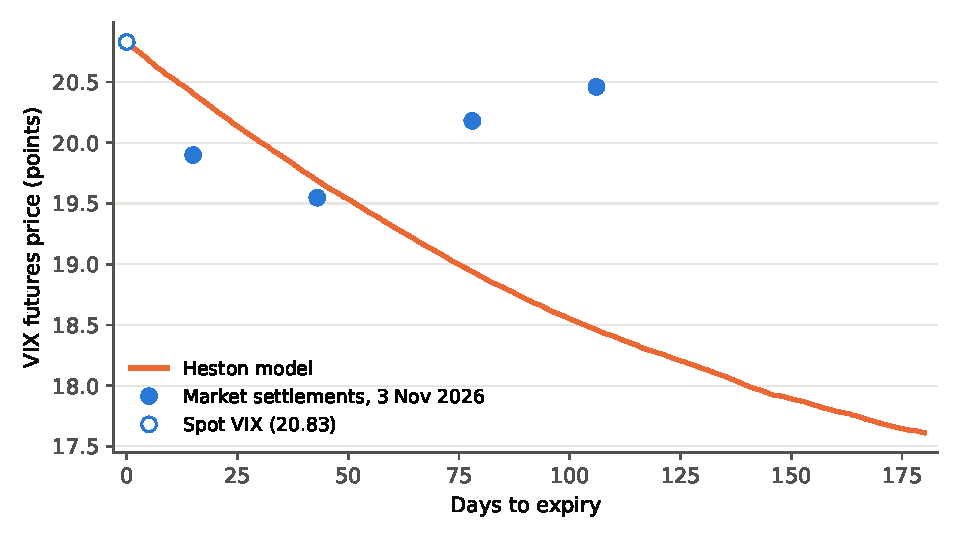
\includegraphics[width=0.85\linewidth]{figures/heston_futures_curve.pdf}
\caption{VIX futures curve on 3 November 2026. Market settlements and the Heston model started at the spot VIX.}
\label{fig:hestoncurve}
\end{figure}

\begin{table}[H]
\centering
\small
\begin{tabular}{@{}lrrrr@{}}
\toprule
\textbf{Expiry} & \textbf{Days} & \textbf{Market} & \textbf{Model} & \textbf{Market $-$ model}\\
\midrule
2026-11-18 & 15 & 19.90 & 20.41 & -0.51 \\
2026-12-16 & 43 & 19.55 & 19.69 & -0.14 \\
2027-01-20 & 78 & 20.18 & 18.94 & +1.24 \\
2027-02-17 & 106 & 20.46 & 18.46 & +2.00 \\
2027-03-17 & 134 & 20.58 & 18.09 & +2.49 \\
2027-04-21 & 169 & 20.93 & 17.70 & +3.22 \\
\bottomrule
\end{tabular}

\caption{VIX futures on 3 November 2026, in VIX points ($\$1{,}000$ per point). Days are calendar days to expiry.}
\label{tab:hestonfutures}
\end{table}

Because $v_0 > \theta$, the model curve falls from 20.83 toward the long run level and reaches 17.6 after 180 days. The market curve is roughly flat, dipping to 19.55 and rising to 20.93. The model is 0.5 points too high at the front and 3.2 points too low at the April contract. There are two reasons. The parameters were fitted to S\&P~500 options, not to VIX futures. And a model with a single variance factor can only move in one direction from today's VIX toward $\theta$, so it cannot produce a curve that dips and then rises. This is a known limitation of such models for VIX futures \cite{bergomi,gatheral2008}.

\subsubsection{VIX call prices}

A VIX call pays $\max(\VIX_T - K, 0)$ at expiry, so its price $C(K,T) = e^{-rT}\,\EQ[\max(\VIX_T - K,0)]$ is the discounted average payoff over the same paths. We discount with the 1 month (30 days) and 3 month (91 days) Treasury yields of 3 November 2026, converted to continuous compounding as in the VIX calculation above. Table~\ref{tab:hestoncalls} lists the prices. One option contract is worth $\$100$ per VIX point.

\begin{table}[H]
\centering
\small
\begin{tabular}{@{}lrrrr@{}}
\toprule
& \multicolumn{2}{c}{\textbf{1 month (30 days)}} & \multicolumn{2}{c}{\textbf{3 months (91 days)}}\\
\cmidrule(lr){2-3}\cmidrule(lr){4-5}
\textbf{Strike} & \textbf{Points} & \textbf{Per contract} & \textbf{Points} & \textbf{Per contract}\\
\midrule
15 & 5.43 & \$543 & 5.26 & \$526 \\
20 & 2.05 & \$205 & 2.59 & \$259 \\
25 & 0.46 & \$46 & 1.03 & \$103 \\
30 & 0.05 & \$5 & 0.33 & \$33 \\
\bottomrule
\end{tabular}

\caption{Heston VIX call prices on 3 November 2026, in VIX points and dollars per contract ($\$100$ per point).}
\label{tab:hestoncalls}
\end{table}

Prices fall as the strike rises. Calls with strikes 20, 25 and 30 are worth more at 3 months, because $\VIX_T$ is more uncertain further out. The call with strike 15 is already well in the money and is worth slightly less at 3 months, because the model's futures price falls from 20.0 to 18.7 between the two dates.
\subsubsection{Convexity adjustment}
\label{sec:hestonconv}

The variance swap replication \eqref{eq:result} shows that option prices fix the price of $\VIX^2$, the variance. A VIX future, however, pays $\VIX$ itself, the square root. If $\VIX_T$ were known for certain, $\sqrt{\EQ[\VIX_T^2]}$ and $\EQ[\VIX_T]$ would be equal. Because $\VIX_T$ is uncertain and the square root is concave, Jensen's inequality makes the first larger. We call the gap the convexity adjustment (CA):
\[
  \mathrm{CA}(T) = \sqrt{\EQ[\VIX_T^2]} - \EQ[\VIX_T] \;\ge\; 0 .
\]
For each date $T$ from 1 to 180 days we compute both terms. $\EQ[\VIX_T^2]$ follows exactly from \eqref{eq:hestonmean} and \eqref{eq:hestonvix}, since $\VIX_T^2$ is linear in $v_T$, and $\EQ[\VIX_T]$ is the simulated futures price. Figure~\ref{fig:hestonconvexity} shows the difference, which is 0.62 points at 30 days, 1.58 at 91 days and 2.28 at 180 days. It grows with maturity because the range of possible values of $\VIX_T$ widens the further ahead we look. This is why a VIX future cannot be priced as the square root of a variance swap.

\begin{figure}[H]
\centering
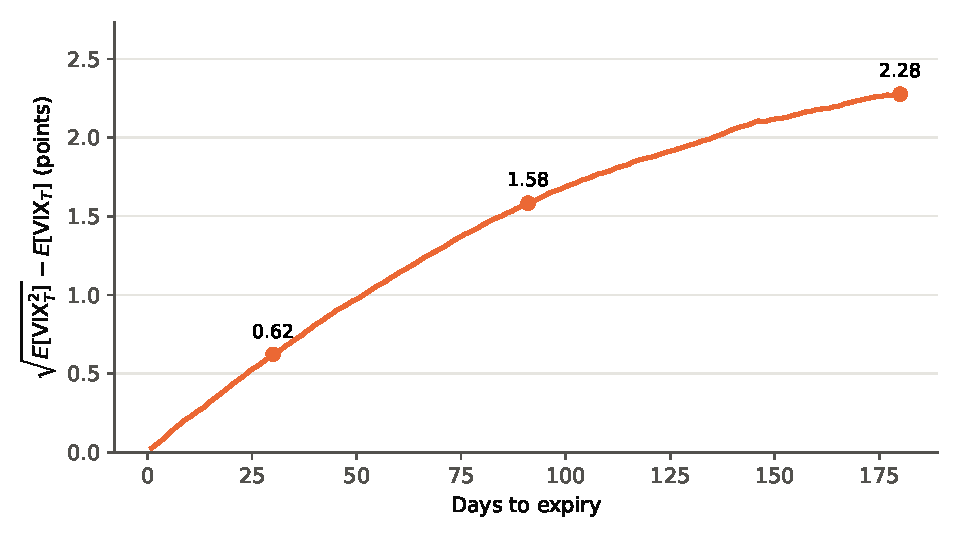
\includegraphics[width=0.85\linewidth]{figures/heston_convexity.pdf}
\caption{Convexity adjustment $\sqrt{\EQ[\VIX_T^2]} - \EQ[\VIX_T]$ under Heston, started at the spot VIX of 3 November 2026.}
\label{fig:hestonconvexity}
\end{figure}

\subsubsection{Limitations}

Heston has a single variance factor, so it ties the whole futures curve to today's VIX and cannot fit a curve that dips and then rises. That would need a second variance factor. Gatheral's parameters were fitted to S\&P~500 options, not to VIX futures or options, and here we adjusted only $v_0$. Daily Euler steps add discretisation error, but the checks against the exact means show it is smaller than the Monte Carlo error.
